\documentclass[12pt, a4paper]{article}
\usepackage[utf8]{inputenc}
\usepackage{amsmath, amssymb, amsthm, amsfonts}
\usepackage{CJKutf8}
\usepackage{tikz}
\usetikzlibrary{arrows.meta, patterns}
\usepackage[margin=1in]{geometry}
\newtheorem{lemma}{Lemma}

 
\newenvironment{solution}
  {\paragraph{\textit{Solution:}}\par\medskip}
  {\hfill$\blacksquare$\vspace{0.1cm}}

\title{Topics in Geometry and Topology:Assignment 2}
\author{
    \begin{CJK*}{UTF8}{gbsn}
    钟皓宇 (12533556)
    \end{CJK*}
}
\date{\today}

\begin{document}

\maketitle

\section*{Problem 1}
If $\Delta$ is a fan in $N$, and $\Delta'$ is a fan in $N'$, show that the set of products $\sigma \times \sigma'$, $\sigma \in \Delta, \sigma' \in \Delta'$, forms a fan $\Delta \times \Delta'$ in $N \oplus N'$, and show that
\[
X(\Delta \times \Delta') = X(\Delta) \times X(\Delta').
\]
\begin{solution}
According to \textit{Homework.1.2}, we already know $\sigma \times \sigma'$ is a rational convex polyhedral cone in $N\oplus N'$. Strong convexity also holds since
\begin{align*}
    -(\sigma\times \sigma')\cap (\sigma\times \sigma')= (-\sigma\cap \sigma)\times (-\sigma'\cap \sigma')=0
\end{align*}
when $\sigma,\sigma'$ are strongly convex. Hence, according to the duality isomorphism
\begin{align*}
    \operatorname{Hom}_{\mathbb{R}}(N_\mathbb{R}\oplus N_\mathbb{R}',\mathbb{R}) \cong \operatorname{Hom}_{\mathbb{R}}(N_\mathbb{R},\mathbb{R}) \oplus \operatorname{Hom}_{\mathbb{R}}(N_\mathbb{R}',\mathbb{R}),
\end{align*}
Any face of $\sigma\times\sigma'$ has the form $(u\times v)^\perp\cap(\sigma\times \sigma')$ where $u\in \sigma^\vee$ and $v\in (\sigma')^\vee$, which implies that faces of $\sigma\times\sigma'$ are cones in $\Delta$
because 
\begin{align*}
    (u\times v)^\perp\cap(\sigma\times \sigma') = (u^{\perp}\cap \sigma) \times (v^{\perp}\cap \sigma'), \tag{$\clubsuit$}
\end{align*}
and $u^{\perp}\cap \sigma,v^{\perp}\cap \sigma'$ as faces of $\sigma,\sigma'$ respectively are contained in $\Delta\times\Delta'$. Suppose $\sigma\times \sigma'$ and 
$\eta\times\eta'$ are two arbitrary cone in $\Delta\times\Delta'$, then the intersection of them
\begin{align*}
    (\sigma\times\sigma')\cap(\eta\times\eta') = (\sigma\cap\eta)\times (\sigma'\cap\eta')
\end{align*}
is the product of two faces $\sigma\cap\eta$ and $\sigma'\cap\eta'$, which are the faces of $\sigma,\eta$ and $\sigma',\eta'$ respectively. 
According to $(\clubsuit)$, this product is also the face of $\sigma\times\sigma'$ and $\eta\times\eta'$. Therefore, $\Delta\times\Delta'$ is a fan
in $N\oplus N'$. To prove the isomorphism of scheme, we need to use the fact that $U_{\sigma\times \sigma'}\cong U_{\sigma}\times U_{\sigma'}$ which have 
proved in \textit{Homework.1.2} and \textbf{Hom-Sheaf}. Specifically, for arbitrary schemes $X$ and $Y$, the assignment
\begin{align*}
    U \mapsto \text{Hom}_{\text{Sch}}(U,Y)
\end{align*}
is a sheaf of sets on $X$, we call it the sheaf of morphisms into $Y$. Therefore, we can construct a morphisms of schemes $f:X(\Delta\times \Delta')\to X(\Delta) \times X(\Delta')$
by glueing of local dates $\{(U_{\sigma\times\sigma'},f_{\sigma\times\sigma'})\}$ where $f_{\sigma\times\sigma'}\in \text{Hom}_{\text{Sch}}(U_{\sigma\times\sigma'},U_\sigma\times U_{\sigma'})$ is 
isomorphism we have obtained. The reason why we can glue is directly because for arbitrary another cone $\eta\times\eta'$,
there exists a cone $\tau\times\tau'\in \Delta\times\Delta'$ such that 
\begin{align*}
    \tau\times\tau' = (\eta\times\eta')\cap (\sigma\times\sigma')
\end{align*}
Scheme-theoretically, this means that
\begin{align*}
    U_{\tau\times\tau'} = U_{\eta\times\eta'} \cap U_{\sigma\times\sigma'}
\end{align*}
and thus 
\begin{align*}
    f_{\eta\times\eta'}|_{U_{\tau\times\tau'}} = f_{\sigma\times\sigma'}|_{U_{\tau\times\tau'}} = f_{\tau\times\tau'}
\end{align*}
which implies local dates $\{(U_{\sigma\times\sigma'},f_{\sigma\times\sigma'})\}$ satisfy the glueing condition. Similarily, we can construct another scheme morphism $g:X(\Delta) \times X(\Delta')\to X(\Delta \times \Delta')$, then we find 
$gf:X(\Delta \times \Delta')\to X(\Delta \times \Delta')$ is identity because we can verify it by restricting to affine open subsets $U_{\sigma\times\sigma'}$ and on each 
\begin{align*}
    gf|_{U_{\sigma\times\sigma'}} = g_{\sigma\times\sigma'}f_{\sigma\times\sigma'}= \text{id}_{U_{\sigma\times\sigma'}}.
\end{align*}
$fg$ is also an identity similarily. Therefore, our discussion validates $X(\Delta \times \Delta') = X(\Delta) \times X(\Delta')$.

\end{solution}

\section*{Problem 2}
Show conversely that any finitely generated sub-semigroup of $M$ that generates $M$ as a group and is saturated has the form $\sigma^\vee \cap M$ for a unique strongly convex rational polyhedral cone $\sigma$ in $N$.

\begin{solution}
    Let $\dim(M_\mathbb{R})= n$.
    Let $S$ be an arbitrary finitely generated sub-semigroup of $M$ such that generates $M$ as a group and is saturated.
    Let $\tau=\mathbb{R}_{\ge 0}\cdot S$ be the subset of $M_{\mathbb{R}}$ generated by $S$ with non-negative real number coefficient.
    Because $S$ is finitely generated, then we suppose that $\{s_1,\cdots,s_n,\dots,s_{m}\}$ are generators of $S$.
    Hence, $S$ generates $M$ implies that $\text{span}\{s_1,\cdots,s_{m}\}=M_{\mathbb{R}}$ and thus 
    $\tau$ can be expressed as 
    \begin{align*}
        \tau = \{r_1s_1+\dots+r_ms_m|r_i\ge 0 \},
    \end{align*}
    which implies $\tau$ is a convex polyhedral cone. Hence, generators $s_i\in M$ implies $\tau$ is rational. 
    I claim that $S = \tau\cap M$ and therefore $S=\sigma^{\vee}\cap M$ if we let $\sigma=\tau^\vee$. 
    If $x\in \tau\cap M$, then I claim that $x$ can be expressed as $x= \sum_{j\in J} y_js_j$ where $J$ is index set such that $\{s_j\}_{j\in J}$ is linearly independent and it forms a basis of $M_{\mathbb{R}}$.
    To see that we can suppose $J$ is the index set such that $\#J= \min\{\# I|I\subseteq \{1,\dots,m\}\text{ for $x\in \mathbb{R}_{> 0}\cdot \{s_i\}_{i\in I}$} \}$. [\textbf{you should notice that we choose the coefficients strictly greater than zero}]If $J$ is not linearly independent, then 
    we can suppose $J=\{1,\dots,j\}$ without loss of generality and suppose $c_1s_1+\dots+c_js_j=0$ with $c_k\neq 0$. Then we consider a new expression
    \begin{align*}
        x =  \sum_{j\in J} (y_j+tc_j)s_j = \sum_{j\in J} y^*_{j} s_j
    \end{align*}
    where we take 
    \begin{align*}
        t = \min_{\{j \in J \mid c_j < 0\}} \left( \frac{y_j}{-c_j} \right)
    \end{align*}
    then there exists $k\in J$ such that $y_k^*=0$, which contradicts to our assumption.
    Next, we extend $J$ to $J'$ such that $\{s_j\}_{j\in J'}$ forms a basis of $M_{\mathbb{R}}$ and $x=\sum_{j\in J'}y_js_j$ with $y_j\ge 0$. Let $y=(y_1,\dots,y_n)^T$ and $A=(s_{ij})_{n\times n}$
    where $s_i = (s_{i1},\dots,s_{in})$ then we obtain that 
    \begin{align*}
        A^T y = x
    \end{align*}
    where the entries of $A,x$ are integers. Therefore, $y = (A^T)^{-1}x$ implies that the entries of $y$ are rational. Hence, there exists a positive integer $d$ such that 
    $dy_j\in \mathbb{Z}$ for all $j\in J'$ and then $dx\in S$ implies $x\in S$ because $S$ is saturated. Then we obtain $S=\tau\cap M = \sigma^{\vee}\cap M$. 
    The strong convexity of $\sigma$ is directly from $S$ generates $M$. If $\tau^\vee=\sigma$ is not strongly convex, then exists $0\neq u\in N$ such that $-u,u\in \sigma$, then $\tau\subseteq u^\perp$ 
    implies $S$ contained in a proper subspace $u^\perp$ cannot generates $M$. To show uniqueness, suppose that $S = \sigma^\vee\cap M=\eta^\vee \cap M$, then we obtain that 
    \begin{align*}
       \sigma^\vee  =  \mathbb{R}_{\ge 0} \cdot (\sigma^\vee\cap M) = \tau = \mathbb{R}_{\ge 0} \cdot (\eta^\vee\cap M)=\eta^\vee,
    \end{align*} 
    and by the isomorphism of double dual we obtain that 
    \begin{align*}
        \sigma = \tau^\vee = \eta.
    \end{align*}
    The uniqueness is validated.
\end{solution}


\section*{Problem 3}
Find the toric varieties corresponding to the following three fans in $\mathbb{Z}^2$:

\vspace{1em}
\begin{center}
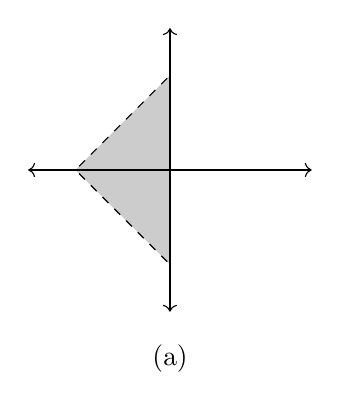
\begin{tikzpicture}[scale=1.2]
    % Fan (a) - 灰度填充 + 虚线边界
    \fill[gray!40] (0,0) -- (-1,0) -- (0,1) -- cycle;
    \fill[gray!40] (0,0) -- (-1,0) -- (0,-1) -- cycle;
    \draw[dashed] (0,0) -- (-1,0) -- (0,1) -- cycle;
    \draw[dashed] (0,0) -- (-1,0) -- (0,-1) -- cycle;
    \draw[<->] (-1.5,0) -- (1.5,0);
    \draw[<->] (0,-1.5) -- (0,1.5);
    \node at (0,-2) {(a)};
\end{tikzpicture}
\hspace{1cm}
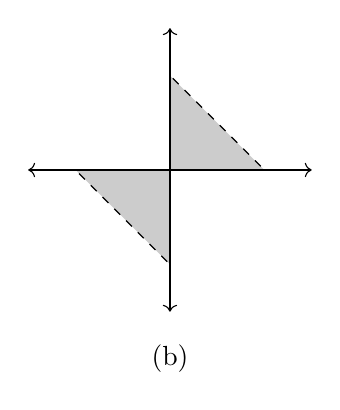
\begin{tikzpicture}[scale=1.2]
    % Fan (b) - 灰度填充 + 虚线边界
    \fill[gray!40] (0,0) -- (1,0) -- (0,1) -- cycle;
    \fill[gray!40] (0,0) -- (-1,0) -- (0,-1) -- cycle;
    \draw[dashed] (0,0) -- (1,0) -- (0,1) -- cycle;
    \draw[dashed] (0,0) -- (-1,0) -- (0,-1) -- cycle;
    \draw[<->] (-1.5,0) -- (1.5,0);
    \draw[<->] (0,-1.5) -- (0,1.5);
    \node at (0,-2) {(b)};
\end{tikzpicture}
\hspace{1cm}
\begin{tikzpicture}[scale=1.2]
    % Fan (c) - 保持原样 (坐标轴)
    \draw[->] (0,0) -- (1.5,0);
    \draw[->] (0,0) -- (0,1.5);
    \node at (0.75,-2) {(c)};
\end{tikzpicture}
\end{center}

\begin{solution}
    \textbf{(a)} Let cones $\sigma,\eta,\tau$ correspond to upper left quadrant, lower left quadrant and negative $x$-axis respectively.
    Then the first fan $\Delta_1$ can be expressed as 
    \begin{align*}
        \Delta_1= \{\sigma,\tau,\eta,0\}.
    \end{align*} 
    Let $\gamma=\mathbb{R}_{\ge 0}$ be the 1-dimensional cone in $\mathbb{R}$. Let $\Delta_1^1 = \{-\gamma,0\}$ and $\Delta_1^2=\{\gamma,-\gamma,0\}$ be two fans 
    in $\mathbb{R}$. Then $\Delta_1 = \Delta_1^1\times \Delta_1^2$ implies that 
    \begin{align*}
        X(\Delta_1)\cong X(\Delta_1^1)\times X(\Delta_1^2) = \mathbb{A}^1_{\mathbb{C}} \times \mathbb{P}^1_{\mathbb{C}}.
    \end{align*}
    \textbf{(b)} Let cones $\sigma_1,\dots,\sigma_4$ correspond to upper right quadrant, upper left quadrant, lower left quadrant and lower right quadrant respectively.
    Let $\Delta = \{\sigma_1,\dots,\sigma_4,\dots\}$ be the fan generated by $\sigma_i$. Then $\Delta = \Delta'\times \Delta'$ where $\Delta' = \{\gamma,-\gamma,0\}$ and $\gamma = \mathbb{R}_{\ge 0}$, which implies 
    $X(\Delta)= \mathbb{P}^1_{\mathbb{C}} \times \mathbb{P}^1_{\mathbb{C}}$. Let $\Delta_2= \{\sigma_1,\sigma_3,\dots\}$ be the fan generated by $\sigma_1,\sigma_3$ which corresponds to the second fan.
    Then $\Delta_2\subseteq \Delta$ implies that $X(\Delta_2)$ is an open subscheme of $\mathbb{P}^1_{\mathbb{C}} \times \mathbb{P}^1_{\mathbb{C}}$ by considering the open immersion defined by glueing the open immersion of open covers of $X(\Delta_2)$.
    Explicitly, we can write 
    \begin{align*}
        f_{\sigma_1}:U_{\sigma_1}\cong \mathbb{A}^2_\mathbb{C} &\to \mathbb{P}^1_{\mathbb{C}} \times \mathbb{P}^1_{\mathbb{C}} \\ (x_1,x_2)&\mapsto ([x_1,1],[x_2,1])
    \end{align*}
    and 
    \begin{align*}
        f_{\sigma_3}:U_{\sigma_3}\cong \mathbb{A}^2_\mathbb{C} &\to \mathbb{P}^1_{\mathbb{C}} \times \mathbb{P}^1_{\mathbb{C}} \\ (y_1,y_2)&\mapsto ([1,y_1],[1,y_2])
    \end{align*}
    where $f_{\sigma_1}$ and $f_{\sigma_3}$ are open immersions and agree on intersection $U_{0}\cong \mathbb{C}^*\times \mathbb{C}^*$. Let $f:X(\Delta_2)\to X(\Delta)$ is 
    the morphism glued by $f_{\sigma_1},f_{\sigma_3}$ then we obtain that 
    \begin{align*}
        X(\Delta_2) \cong \text{Im}(f) = (\mathbb{P}^1_{\mathbb{C}} \times \mathbb{P}^1_{\mathbb{C}})\backslash \{(\infty,0),(0,\infty)\}.
    \end{align*}
    \textbf{(c)}  Similarily, let $\sigma_1$ be the cone correspond to upper right quadrant and $\Delta=\{\sigma_1,\cdots,\}$ be the fan generated by $\sigma_1$.
    We consider the open immersion induced by $\Delta_3\subseteq \Delta$, where $\Delta_3$ is the third fan with cones $x$-axis $\sigma_x$ and $y$-axis $\sigma_y$.
    Then we have open immersions $f$ glued by 
    \begin{align*}
        f_{\sigma_x}: U_{\sigma_x}\cong \mathbb{A}_{\mathbb{C}}^1 \times \mathbb{C}^* &\to \mathbb{A}_{\mathbb{C}}^2 \\
        (a,c) &\mapsto (a,c) 
    \end{align*}
    and 
        \begin{align*}
        f_{\sigma_y}: U_{\sigma_y}\cong \mathbb{C}^*  \times  \mathbb{A}_{\mathbb{C}}^1&\to \mathbb{A}_{\mathbb{C}}^2 \\
        (c,a) &\mapsto (c,a) 
    \end{align*}
    Therefore we obtain that $X(\Delta_3)\cong \text{Im}(f)=\mathbb{A}^2_{\mathbb{C}} \backslash \{(0,0)\}$.
\end{solution}
\section*{Problem 4}
Show that if $X(\Delta)$ is an affine variety, then $\Delta$ consists of all faces of some cone $\sigma$, so $X(\Delta) = U_\sigma$.
\begin{solution}
    Suppose $\dim(X(\Delta))= n$.
    Since $X(\Delta)$ is affine, it follows there exists a commutative ring $R$ such that $X(\Delta)\cong \text{Spec}(R)$.
    We claim that every ideal $I$ of $R$ corresponding to a $T_N$-invariant closed subscheme of $X(\Delta)$ is graded.
    The open immersion $T_N\hookrightarrow X(\Delta)$ induced the injection $R \hookrightarrow (\mathbb{C}^*)^n$ because 
    $X(\Delta)$ is integral. The ideal $I$ can be regarded as the subset of $(\mathbb{C}^*)^n$. Suoppose $f=\sum a_m\chi^m$ is an arbitrary element of ideal $I$.
    The torus $T_N$ acts on $I$ by sending $f$ to 
    \begin{align*}
        t \cdot f = \sum_{m \in S} a_m (t \cdot \chi^m) = \sum_{m \in S} \left( a_m \chi^m(t^{-1}) \right) \chi^m \tag{$\clubsuit$}
    \end{align*}
    where $S$ is the index set of coefficients $a_m$ and the last step of $(\clubsuit)$ is given by
    \begin{align*}
        t.\chi^m(z) = \chi^m (t^{-1}z) = \chi^m(t^{-1})\chi^m(z) \tag{$\spadesuit$}
    \end{align*}
    where $z$ be an arbitrary closed point of $X(\Delta)$ and $\chi^m$ as a character of representations, alternatively, closed points $\text{Hom}_{\text{Ring}}(R,\mathbb{C})$ yields the last step of ($\spadesuit$).
    Suppose $\# S = r$. The linear independence of characters implies there exists $t_1,\dots,t_r$ such that $r\times r$ matrix $(\chi^{m_i} (t_j))$ is invertible.
    If not, it means that $\{\chi^m\}_{m\in S}$ is linear dependence on torus $T_N$. 
    Since torus is the open dense subscheme of $X(\Delta)$, which implies a contradiction that $\{\chi^m\}_{m\in S}$ is linear dependence on $X(\Delta)$.
    Define $f_i= t_i.f$, let $F=(f_1,\cdots,f_r)^T$, $A=(\chi^{m_i} (t_j))$ and $X=(a_1\chi^{m_1},\cdots,a_r\chi^{m_r})$. We obtain that $F=AX$. Since $A$ is invertible then we have $X=A^{-1}F$.
    Hence, $I$ is $T_N$ invariant implies that $f_i\in I$ and therefore every entries of $X$ is contained in $I$. Equivalently, $I$ is graded.  
    

\end{solution}


\end{document}